\section{Modelo}
\subsection{Descripción del Entorno Biológico.}

Considérese un organismo con acceso a dos recursos para su supervivencia. Sean $S_1$ y $S_2$ las concentraciones de estos dos recursos contenidos en un chemostat. Entonces el vector:
\begin{equation}
	I=\binom{S_{1}}{S_{2}},
\end{equation}

constituye la condición ambiental para el consumidor.\citep{Diekmann2001, diekman2003}.

Ahora bien, estos organismos pueden especializarse de mayor o menor medida en el consumo de cualquiera de los 2 recursos a su disposición. Describimos esto en un rasgo cuantizable $x$ que varía continuamente entre $[0,1]$. Si $x$ equivale a 0, sólo el recurso $S_2$ es consumido, caso contrario cuando equivale 1, sólo se consume el recurso $S_1$. Extendiendo a escala poblacional, el impacto causado por el rasgo $x$ se toma implícitamente dentro de los coeficientes $\eta(x)$ y $\xi(x)$, definidos de tal manera que la proporción de ingesta \textit{per cápita} de un solo organismo con rasgo $x$ equivale, respectivamente a: $\eta(x)$ $S_1$ y $\xi(x)$ $S_2$.\citep{dieckman2005}

En el caso de una población monomórfica, la dinámica ecológica está gobernada por el siguiente sistema de ecuaciones diferenciales:
\begin{equation}\label{eqmono}
	\begin{split}
		\frac{d S_1}{dx} & =S_{01}-S_1-\eta(x)S_1X \\  \frac{d S_2}{dx}&=S_{02}-S_2-\xi(x)S_2X\\ \frac{d X}{dx}&=-X+\eta(x)S_1X+\xi(x)S_2X
	\end{split}
\end{equation}

Donde X representa la densidad de la población consumidora y $S_{01}$ es la concentración del recurso i ($i\in\{1,2\}$) en el medio de entrada, para este modelo, la tasa de crecimiento poblacional de los consumidores con el rasgo $x$ bajo condiciones ambientales estables $I$ ($\frac{d X}{dx}=0$ en la tercera expresión de \eqref{eqmono}), está dada por:
\begin{equation}\label{r}
	\begin{split}
		0      & =r(x,I)X                  \\
		r(x,I) & =-1+\eta(x)S_1+\xi(x)S_2.
	\end{split}
\end{equation}

Por lo tanto la primera condición para estados estables es:
\begin{equation*}
	r(x,I)=0
\end{equation*}

Para las 2 primeras expresiones de \eqref{eqmono} obtenemos lo siguiente para las mismas condiciones de estabilidad:
\begin{equation*}
	\begin{split}
		0 & =S_{01}-S_1-\eta(x)S_1X \\  0&=S_{02}-S_2-\xi(x)S_2X
	\end{split}
\end{equation*}
Con la que, obteniendo $S_1$ y $S_2$ en términos de $X$ y sustituyendo en nuestra primera condición de estabilidad $r=0$ tenemos:

\begin{equation*}
	-1+\frac{\eta(x)S_{01}}{1+\eta(x)X}+\frac{\xi(x)S_{02}}{1+\xi(x)X}=0
\end{equation*}

Que es una función monótona decreciente de $X$ con límite -1 para $X\to\infty$, y que tiene solución positiva para X=0 solo si:
\begin{equation}\label{global}
	\eta(x)S_{01}X+\xi(x)S_{02}X>1,
\end{equation}
entonces \eqref{eqmono} tiene un único estado estable no trivial que es asintótico globalmente, dado que cumpla \eqref{global}.

\subsection{Sistemas de Ecuaciones de Selección-Mutación y Paso al Límite para Mutaciones.}

Si la reproducción no es completamente fiel (aparece alguna mutación), un consumidor con el rasgo $y$ puede generar descendencia con el rasgo $x$. Sea $K(x,y)$ la densidad de probabilidad correspondiente. Sea $n(t,.)$ la densidad de consumidores en el tiempo t. El sistema \citep{dieckman2005}:

\begin{equation}\label{core}
	\begin{split}
		\frac{d S_1}{dt}(t) & =S_{01}-S_1(t)-S_1(t)\int_{0}^{1}\eta(y)n(t,x)dx,                \\
		\frac{d S_1}{dt}(t) & =S_{02}-S_2(t)-S_2(t)\int_{0}^{1}\xi(x)n(t,x)dx                  \\
		\frac{d n}{dt}(t,x) & =-n(t,x)+\int_{0}^{1}K(x,y)[S_1(t)\eta(y)+S_2(t)\xi(x)]n(t,y)dy,
	\end{split}
\end{equation}

describe la interacción, a través de los recursos, de los diversos tipos de consumidores, así como el efecto de la mutación, le denominaremos sistema de ecuaciones de selección-mutación. Tomamos que la descendencia de un individuo con el rasgo $x$ tiene una distribución de rasgos descrita por la densidad $K(x,.)$.

Además, asumiendo que las mutaciones son muy pequeñas, de tal manera que la distribución de probabilidad $K(x,y)$ es muy pequeño para $x$ fuera de un vecindario de radio $\varepsilon$ con ''centro'' en $y$, $\varepsilon>0$ muy pequeño, entonces tomamos $K(x,y)\to K_{\varepsilon}(x,y)$ dependiente de este pequeño parámetro $\varepsilon$.\citep{dieckman2005}

Reescalamos el tiempo sustituyendo $\tau=\varepsilon$t (este escalamiento ajusta la escala temporal de modo que, al hacer $\varepsilon$ desaparecer, la escala de tiempo se adapte para observar el efecto de las mutaciones), reescribimos \eqref{core}:

\begin{equation}\label{nocon}
	\frac{\varepsilon}{n(\tau,x)}\frac{d n(\tau,x)}{d\tau}=-1+\int_{0}^{1}K(x,y)_{\varepsilon}[S_1(\tau)\eta(y)+S_2(\tau)\xi(x)]\frac{n(y,\tau)}{n(\tau,x)}dy.
\end{equation}

a la que a la vez podemos luego realizar la siguiente transformación

\begin{equation*}
	\varphi(\tau,x)=\varepsilon ln[n(\tau,x)],
\end{equation*}
entonces:
\begin{equation*}
	\frac{d\varphi(\tau,x) }{d\tau}=\int_{0}^{1}K_{\varepsilon}(x,y)[S_1(\tau)\eta(y)+S_2(\tau)\xi(x)]e^{\frac{\varphi(\tau,y)-\varphi(\tau,x)}{\varepsilon}}dy
\end{equation*}

Aprovechando lo mencionado anteriormente sobre $K_{\varepsilon}(x,y)$ realizamos el cambio de variable de integración $y=x+\varepsilon z$ y de la definición de derivada parcial:

\begin{equation*}
	\frac{\varphi(\tau,y)-\varphi(\tau,x)}{\varepsilon} \to \frac{d\varphi(\tau,x) }{dx}z
\end{equation*}

y asumimos que la probabilidad de aparición de un nuevo rasgo como resultado de una mutación depende únicamente de la distancia al rasgo original. Por lo tanto, reemplazamos el kernel $K_{\varepsilon}$ por un kernel de convolución $\widetilde{K}$:

\begin{equation*}
	K_{\varepsilon}(x,y)dy\longrightarrow \widetilde{K}(z)dz
\end{equation*}

Donde $\widetilde{K}$ es una función no negativa y par definida en $(-\infty,+\infty)$, cuya integral es igual a 1. Al tomar formalmente el límite cuando $\varepsilon\to 0$ en \eqref{nocon}, obtenemos:

\begin{equation}\label{hj}
	\frac{d\varphi(t,x) }{dx}=-r(x,I)+[S_1(t)\eta(y)+S_2(t)\xi(x)]\Ham(\frac{\partial \varphi(t,x) }{\partial x})
\end{equation}

la ecuación de Hamilton-Jacobi, dónde r se define en \eqref{r} y $\Ham$ se toma como:
\begin{equation*}
	\Ham(p)=\int_{-\infty}^{\infty}\widetilde{K}(z)e^{-pz}dz-1
\end{equation*}

y que cumple $\Ham(0)=0$ y que, para una función par $\widetilde{K}$, $\Ham'(0)>0$; por lo tanto, $\Ham$ es convexa. Llamamos a $\Ham$ el Hamiltoniano correspondiente a $\widetilde{K}$.

\subsection{Descripción del Método numérico}
\subsubsection{Diferencias finitas}

Es un método numérico para la solución de ecuaciones diferenciales, se basa en la discretización de las variables dependientes e independientes convirtiendo las ecuaciones continuas en sistemas algebraicos más fáciles de resolver.

Es una técnica útil para la solución de sistemas complejos. Consiste en aproximar las derivadas de las ecuaciones mediante \textbf{diferencias finitas}, esto es, que se reemplaza la derivada de una función en términos continuos por una expresión algebraica que involucra a la función en puntos discretos en una malla de tiempo, espacio, etc.

\textbf{{Cómo funciona el Método de Diferencias Finitas}}
\begin{enumerate}
	\item Discretización.

	      Se discretizan las variables independientes en una malla, y las soluciones se calculan en algún punto de la malla

	\item Aproximación de Derivadas

	      Las derivadas de las funciones se reemplazan por diferencias finitas en cada punto de la malla. Este reemplazo se hace dependiendo del problema

	\item Ecuaciones algebraicas

	      Al reemplazar las derivadas por diferencias finitas, se obtienen ecuaciones algebraicas fáciles de resolver

	\item Iteración

	      El sistema de ecuaciones se resuelve de manera iterativa, los valores de la solución en cada punto de la malla se calculan por pasos hasta obtener una solución en todo el dominio
\end{enumerate}

Este método presenta algunas ventajas y desventajas: simplicidad ya que es fácil de implementar, aplicación, es aplicable a problemas de difusión, reacción, etc. Por otro lado, tiene como inconveniente que: el error es inversamente proporcional al tamaño de la malla, pero si se hace la malla más pequeña, tiene más costo computacional, si los pasos temporales son grandes, esto puede ocasionar que la solución no sea estable\footnote{Que el método sea inestable se refiere a que el error en la solución crece conforme el tiempo}\citep{ledesma2015introduccion}.

\subsubsection{Diferencias finitas Semi-Implicito}

Se usa para la solución de sistemas de ecuaciones diferenciales en los que aparecen fenómenos de difusión y reacción. Es un método que involucra la solución combinando dos métodos explicito e implícito, y el método es estable\citep{Monteiro2024}.

\textbf{Explicito:} las variables en el paso de tiempo se calculan en el paso actual con la información del paso anterior, este es inestable en algunas ecuaciones.

\textbf{Implícito:} las variables en el paso de tiempo se calculan en el siguiente paso, este es más costoso computacionalmente, pero es más estable

\subsection{Aplicación a la ecuación de Selección-Mutación}
Se presentan los modelos para simulación numérica de la ecuación \eqref{core} Selección-Mutación, y \eqref{hj} la aproximación Hamilton-Jacobi \citep{dieckman2005}.

La ecuación de Selección-Mutación \eqref{core} de forma discreta para la implementación de diferencias finitas semi implícitas es
\begin{equation}
	\left\{
	\begin{aligned}
		\label{eq:dis}
		S_{i}^{(k+1)} & = S_{i}^{0}-\Delta tS_{i}^{(k+1)}[1+\langle{n^{(k)}\eta_{i}}\rangle]                                          \\
		n_{j}^{(k+1)} & = n_{j}^{(k)}-\Delta t n_{j}^{(k+1)}+\Delta t([S_{1}^{(k+1)}\eta+S_{2}^{(k+1)}\xi]n^{(k)}\star \tilde{K})_{j}
	\end{aligned}
	\right.
\end{equation}

donde
\begin{equation*}
	\langle{n^{(k)}\eta_{i}}\rangle = \frac{1}{N}\sum_{j=1}^{N}n_{j}^{(k)}\eta_{j}
\end{equation*}

\begin{equation*}
	(\eta n^{(k)}\star \tilde{K})_{j}=\frac{1}{2M+1}\sum_{m=-M}^{M}\eta_{j-m}n_{j-m}^{(k)}\tilde{K}_{M}
\end{equation*}

donde $\Delta t$ es el paso de tiempo, y $t^k=k\Delta t$, los exponentes representan el paso de tiempo, los indices $i=1,2$ representan los nutrientes, $j$ es la posición en la malla de las diferencias finitas, $\tilde{K}$ es el kernel convolucional de mutación.

El primer término de la \eqref{eq:dis} representa la dinámica de los nutrientes, el segundo término se refiere a la dinámica de los consumidores, $\langle{n^{(k)}\eta_{i}}\rangle$ es el promedio de la densidad de consumidores por su capacidad de consumir uno de los nutrientes, y $(\eta n^{(k)}\star \tilde{K})_{j}$ es la operación de convolución, este modula las interacciones de los consumidores en el espacio discreto del rasgo $x$, $y$

La aproximación de Hamilton-Jacobi de forma discreta es la siguiente:

\begin{equation}
	\left\{
	\begin{aligned}
		\label{HJ_dis}
		\varphi_{j}^{(k+1)}                   & =\varphi_{j}^{(k)}+\Delta t\left[ -1+[S_{1}^{(k)}\eta_{j}+S_{2}^{(k)}\xi_{j}]\left[ 1+\mathcal{H}\left( \frac{\varphi_{j+1}^{(k)}-\varphi_{j}^{(k)}}{\Delta x};\frac{\varphi_{j}^{(k)}-\varphi_{j-1}^{(k)}}{\Delta x} \right) \right] \right] \\
		\max_{1\leq j\leq N}\varphi_{j}^{(k)} & =0\:\:\: \forall k
	\end{aligned}
	\right.
\end{equation}
la solución de este sistema requiere un solucionador "upwind" para el Hamiltoniano, y tiene por dificultad satisfacer las constricciones, esto se soluciona mediante
\begin{equation*}
	S^{(k)} = \min_{1\leq m\leq N}\sum_m^{(k)}
\end{equation*}

\subsection{Experimento numérico}
Mediante la aplicación de los modelos numéricos es posible tener una idea de la dinámica de la densidad de la población en el tiempo y como cambia el rasgo dependiendo de las condiciones del ambiente y la población.

Para la experimentación numérica, se usan los siguientes parámetros: $\tilde{K}_m:=1$, una función constante de $1$, $N=1500$ puntos para la simulación directa y $200$ para la aproximación, $M=5$\citep{dieckman2005}.

La aplicación de los modelos se realiza de dos formas, la primera en que tenemos un ambiente inicial con dos nutrientes en la misma cantidad, y un consumidor con una densidad de población mas especializada en el consumo del nutriente $2$, se elimina el segundo nutriente y se realiza el experimento Figura~\ref{sim1}. El segundo experimento tenemos los dos nutrientes y una densidad de población inicial mas especializada al consumo del nutriente dos Figura~\ref{sim2}.

\begin{figure}[H]
	\centering
	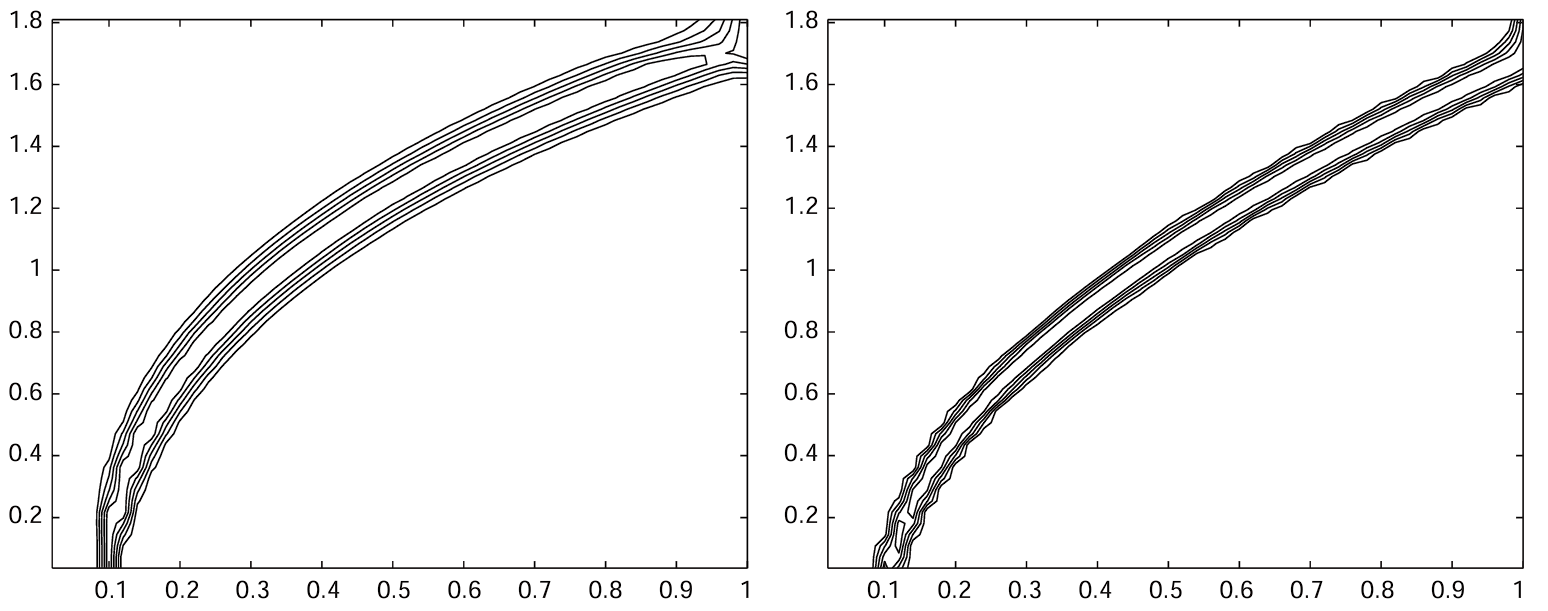
\includegraphics[scale=0.4]{image.png}
	\caption{Primera simulación. El eje $x$ es la característica y el eje $y$ es el tiempo. La población se especializa al consumo del primer nutriente ($\eta(x)=1/1-x$)\citep{dieckman2005}}
	\label{sim1}
\end{figure}

\begin{figure}[H]
	\centering
	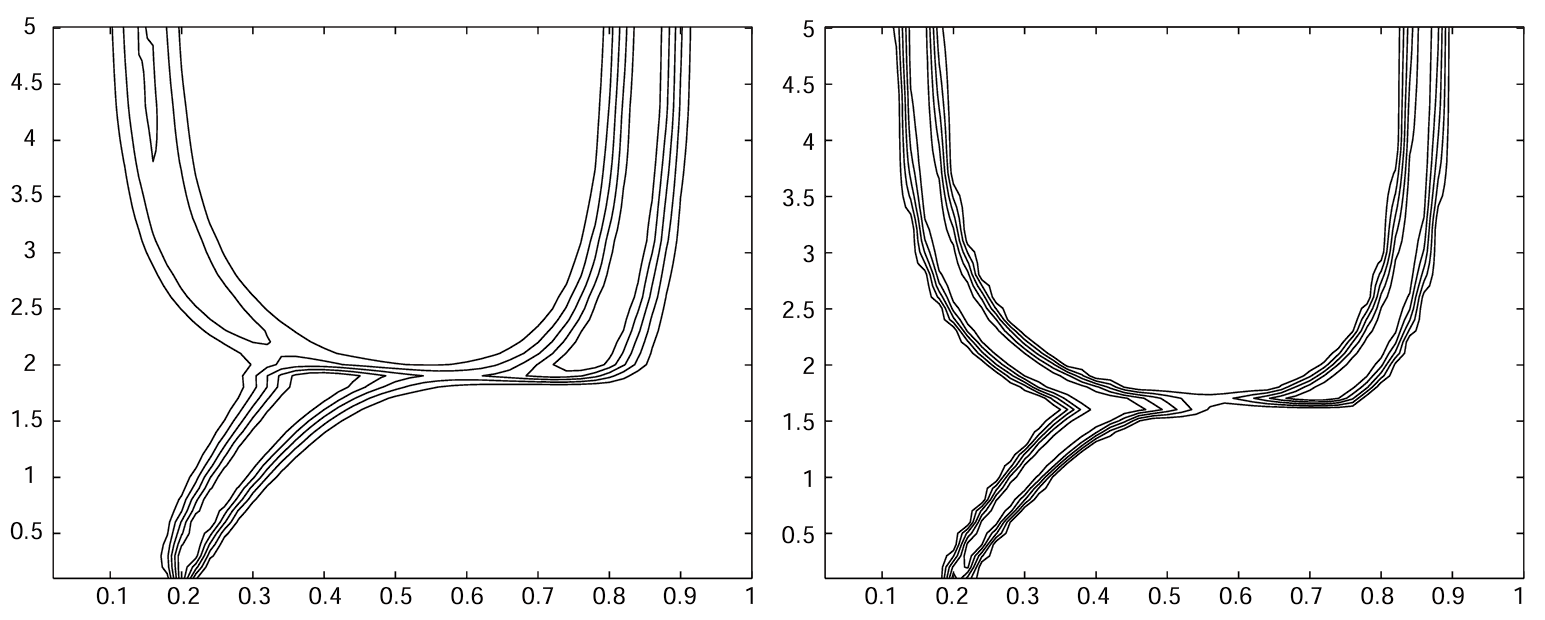
\includegraphics[scale=0.4]{Captura de pantalla 2024-12-11 095132.png}
	\caption{Segunda simulación. El eje $x$ es la característica y el eje $y$ es el tiempo. La especialización en el consumo se divide en dos dando una ramificación ($\eta(x)=x-1.8x(1-x)[x(1-x)-6/25]$, $\xi=1-x-1.8x(1-x)[x(1-x)-6/25]$)\citep{dieckman2005}}
	\label{sim2}
\end{figure}
Las gráfica Figura~\ref{sim1} y Figura~\ref{sim2} representan las líneas de nivel de la densidad de población en el espacio característica-tiempo.
\subsection{Resultados}
A partir del experimento numérico, se pueden ver varios resultados importantes que ayudan a comprender la dinámica de la población y su adaptación al ambiente.

Para el primer experimento encontramos:

\begin{enumerate}
	\item Tendencia hacia $x=1$: La densidad de la población muestra una inclinación hacia $x=1$, esto nos dice que, a medida que transcurre el tiempo, la población adapta su consumo para depender del nutriente 1, que es el único disponible. Este fenómeno refleja cómo las condiciones del ambiente obligan a la población a maximizar su supervivencia a través de un consumo más eficiente del recurso. Este comportamiento puede interpretarse como el efecto de un "potencial" ambiental que dirige la evolución adaptativa de la población hacia un estado óptimo.
	\item Estabilidad en tiempos largos: Conforme el tiempo avanza, la población parece alcanzar un estado de equilibrio en su densidad. La mayor parte de la población depende del nutriente 1.
	\item Forma logarítmica en el movimiento de la densidad: la trayectoria del movimiento de la densidad parece tener un comportamiento logarítmico, que empieza un crecimiento rápido de la adaptación y se va reduciendo a medida que la población se acerca al estado de equilibrio, la adaptación de una especie a su entorno, no presenta un comportamiento lineal en el tiempo.
\end{enumerate}

\textbf{Analogía con el movimiento de un frente de onda:} El movimiento de la densidad de la población en el espacio definido por la característica $x$ y el tiempo presenta una analogía interesante con la propagación de un frente de onda. Este frente parece desplazarse en la dirección positiva de $x$ a medida que el tiempo avanza, es similar a un frente de onda en un medio físico. Este enfoque permite interpretar el comportamiento de la densidad no solo como un proceso adaptativo, sino también como un fenómeno de propagación en este espacio.

Para el segundo experimento (con dos nutrientes) encontramos:
\begin{enumerate}
	\item Estabilidad y eficiencia en el consumo:
	      La densidad de la población muestra una tendencia a alcanzar la estabilidad y a maximizar la eficiencia en el consumo de los recursos disponibles. Esto refleja un comportamiento adaptativo general de la población frente a las condiciones del entorno.

	\item Aparición de un efecto de competencia:
	      La disponibilidad de dos nutrientes genera un fenómeno de competencia entre los miembros de la población. Como resultado, la población adapta su consumo dividiéndose en dos grupos: uno que se especializa en el consumo del nutriente 1 y otro que se especializa en el nutriente 2. Creemos que esta división es impulsada por la necesidad de optimizar el consumo y repartir los recursos de manera más eficiente, minimizando la competencia interna, esto hace posible formular este comportamiento en términos de un principio variacional.

	\item Especialización de las sub-densidades
	      Tras la división, las dos partes de la densidad de población (que, aunque forman parte de la misma población, pueden considerarse característicamente distintas) se especializan en el consumo de uno de los dos nutrientes. Este comportamiento permite una distribución más eficiente de los recursos en el sistema, reforzando la estabilidad del ambiente y la población.
\end{enumerate}

\textbf{Analogía como efecto de dispersión:}
A partir de la analogía con un frente de onda, observamos que el sistema genera un efecto que separa las densidades hacia $x=1$ y $x=0$, reflejando la especialización hacia cada uno de los nutrientes. Sin embargo, no podemos interpretar este comportamiento estrictamente como un fenómeno de onda, ya que no se observan características típicas de las ondas como la difracción, donde las superposiciones podrían generar efectos constructivos o destructivos. En lugar de ello, el sistema parece mostrar un efecto más cercano a un fenómeno de dispersión, en el que las densidades se separan sin interferencias mutuas significativas, y donde el parámetro de impacto parece estar dado por las características del consumo de los nutrientes, funciones $\eta(x),\:\xi(x)$.